%%%%%%%%%%%%%%%%%%%%%%%%%%%%%%%%%%%%%%%%%
% Short Sectioned Assignment
% LaTeX Template
% Version 1.0 (5/5/12)
%
% This template has been downloaded from:
% http://www.LaTeXTemplates.com
%
% Original author:
% Frits Wenneker (http://www.howtotex.com)
%
% License:
% CC BY-NC-SA 3.0 (http://creativecommons.org/licenses/by-nc-sa/3.0/)
%
%%%%%%%%%%%%%%%%%%%%%%%%%%%%%%%%%%%%%%%%%

%----------------------------------------------------------------------------------------
%	PACKAGES AND OTHER DOCUMENT CONFIGURATIONS
%----------------------------------------------------------------------------------------

\documentclass[paper=a4, fontsize=11pt]{scrartcl} % A4 paper and 11pt font size
\usepackage[brazilian]{babel}
\usepackage[utf8]{inputenc}
\usepackage[T1]{fontenc}
\usepackage{amsmath,amsfonts,amsthm,mathtools} % Math packages
\usepackage{xspace}
\usepackage{indentfirst}
\usepackage{placeins}
\usepackage{graphicx,subcaption}
\usepackage{amssymb}
\usepackage{tikz}
\usetikzlibrary{arrows}
\usetikzlibrary{positioning}
\usetikzlibrary{calc}

%\usepackage{sectsty} % Allows customizing section commands
%\allsectionsfont{\centering \normalfont\scshape} % Make all sections centered, the default font and small caps

\usepackage{fancyhdr}
\pagestyle{fancyplain}
%\fancyhead{}
\fancyfoot[L]{} % Empty left footer
\fancyfoot[C]{} % Empty center footer
\fancyfoot[R]{\thepage} % Page numbering for right footer
\renewcommand{\headrulewidth}{0pt} % Remove header underlines
\renewcommand{\footrulewidth}{0pt} % Remove footer underlines
\setlength{\headheight}{13.6pt} % Customize the height of the header

\bibliographystyle{apalike}

%\sectionfont{\bfseries\Large\raggedright}
%\subsectionfont{\bfseries\Large\raggedright}

\newtheorem{theorem}{Teorema}
\newtheorem{definition}{Definição}
\newtheorem{property}{Propriedade}
\newtheorem{proposition}{Proposição}

\newenvironment{example}[1][Exemplo]{\begin{trivlist}
\item[\hskip \labelsep {\bfseries #1}]}{\end{trivlist}}
\newenvironment{exerc}[1][Exercício]{\begin{trivlist}
\item[\hskip \labelsep {\bfseries #1}]}{\end{trivlist}}

\numberwithin{equation}{subsection}
\numberwithin{figure}{subsection}
\numberwithin{table}{subsection}
\numberwithin{definition}{subsection}
\numberwithin{theorem}{subsection}
\numberwithin{property}{subsection}
\numberwithin{proposition}{subsection}
%\numberwithin{example}{subsection}

\numberwithin{equation}{section}
\numberwithin{figure}{section}
\numberwithin{table}{section}
\numberwithin{definition}{section}
\numberwithin{theorem}{section}
\numberwithin{property}{section}
\numberwithin{proposition}{section}
%\numberwithin{example}{section}


% Default fixed font does not support bold face
\DeclareFixedFont{\ttb}{T1}{txtt}{bx}{n}{12} % for bold
\DeclareFixedFont{\ttm}{T1}{txtt}{m}{n}{12}  % for normal

% Custom colors
\usepackage{color}
\definecolor{deepblue}{rgb}{0,0,0.5}
\definecolor{deepred}{rgb}{0.6,0,0}
\definecolor{deepgreen}{rgb}{0,0.5,0}

\usepackage{listings}

% Python style for highlighting
\newcommand\pythonstyle{\lstset{
language=Python,
basicstyle=\ttm,
otherkeywords={self},             % Add keywords here
keywordstyle=\ttb\color{deepblue},
emph={MyClass,__init__},          % Custom highlighting
emphstyle=\ttb\color{deepred},    % Custom highlighting style
stringstyle=\color{deepgreen},
frame=tb,                         % Any extra options here
showstringspaces=false            % 
}}

% Python environment
\lstnewenvironment{python}[1][]
{
\pythonstyle
\lstset{#1}
}
{}


%\setlength{•}{•}\parindent{0pt} % Removes all indentation from paragraphs - comment this line for an assignment with lots of text

%----------------------------------------------------------------------------------------
%	TITLE SECTION
%----------------------------------------------------------------------------------------

\newcommand{\horrule}[1]{\rule{\linewidth}{#1}} % Create horizontal rule command with 1 argument of height

\title{	
\normalfont \normalsize 
\textsc{Modelos Probabilísticos Baseados em Grafos} \\ 
\textsc{Prof. Denis Mauá} \\ [25pt]
%\horrule{0.5pt} \\[0.4cm] % Thin top horizontal rule
\huge Separação Direcional \\ em \\ Redes Bayesianas\\ [25pt]
%\horrule{1pt} \\[0.5cm] % Thick bottom horizontal rule
}
\author{Thales A. B. Paiva \\ thalespaiva@gmail.com} % Your name
\date{\today} % Today's date or a custom date

\renewcommand{\P}{\mathbb{P}}
\renewcommand{\bar}[1]{\overline{#1}}
\newcommand{\set}[1]{\mathcal{#1}}

\def\ind{\perp\!\!\!\perp}
\def\nind{\not\!\perp\!\!\!\perp}

\begin{document}


\maketitle % Print the title
\horrule{1pt} \\[0.5cm] % Thick bottom horizontal rule

\tableofcontents

\pagebreak
\section{Separação Direcional}
\FloatBarrier

Queremos um meio sistemático de determinar quando um conjunto de variáveis $\set{X}$ é condicionalmente independente de outro $\set{Y}$, dado um conjunto $\set{Z}$ de variáveis observadas. Simbolicamente, queremos decidir se $ \set{X} \ind \set{Y} | \set{Z}$, ou se $ \set{X} \nind \set{Y} | \set{Z}$, dados cada um desses conjuntos de variáveis. 

Um modo de atacar este problema é estudar quando há troca de informação entre dois nós de uma rede bayesiana (usarei nó e variável como sinônimos). Ou seja, dadas duas variáveis, como determinamos se duas delas são condicionalmente independentes apenas olhando para a topologia de seu digrafo de dependência. O motivo de nos preocuparmos com a topologia da rede, é que as relações de independência descobertas desta forma devem valer para todas as distribuições de probabilidade que fatoram esta rede.

Considere os nós $X$, $Y$, $Z$. Para o caso em que há um arco $X \rightarrow Y$, é claro que não é para qualquer distribuição que a independência $X \ind Y | Z$ vale. Então, vamos considerar os digrafos mais simples em que $X$ e $Y$ interagem indiretamente através de $Z$. Estes digrafos são as 4 possíveis trilhas entre $X$ e $Y$ com $Z$ entre eles. Lembre que uma trilha em um digrafo é apenas um caminho em seu grafo induzido pela eliminação das orientações das arestas. As trilhas de interesse podem ser vistas na Figura~\ref{fig:trilhas}.

Dizemos que uma trilha $X \leftrightharpoons Z \leftrightharpoons Y$ é ativa se há troca de informação entre $X$ e $Y$ através de $Z$. Vejamos, intuitivamente, quando uma trilha é necessariamente inativa, ou construir casos em que ela pode ser ativa (para \emph{quase todas} as distribuições que fatoram a rede).

\begin{description}
  \item \textbf{Causal} [\ref{fig:trilha_causal}] Suponha que a variável $Z$ foi observada na trilha $X \rightarrow Z \rightarrow Y$. Então uma informação sobre $X$ não deve afetar nossas crenças sobre $Y$ pois, numa rede bayesiana, $X$ é condicionalmente independente dos não descendentes de $X$, dados os seus pais ($X \ind nd(X) | pa(X)$). Agora suponha que a variável $Z$ não foi observada. Então uma informação sobre $X$ nos dá informação sobre $Z$, e esta nos dá informação sobre $Y$. Assim, nossa trilha causal é ativa se $Z$ não for observada, e inativa caso contrário.
  
  \item \textbf{Evidencial} [\ref{fig:trilha_evidencial}] Por uma argumentação similar à do caso anterior, uma trilha evidencial $X \leftarrow Z \leftarrow Y$ é ativa se $Z$ não for observada, e inativa caso contrário.

  \item \textbf{Causa Comum} [\ref{fig:trilha_cc}] Considere a trilha de causa comum $X \leftarrow Z \rightarrow Y$ e suponha que $Z$ é variável observada. Temos que:
  $X \ind nd(X) | pa(X) \Rightarrow X \ind Y | Z$ e portanto a trilha é inativa. Agora, se $Z$ não for observada, informação sobre $Y$ pode sugerir informação sobre $Z$, que por sua vez é propagada para $X$. Como exemplo, considere o caso em que $Z = \text{Aline sente frio}$, $X = \text{Aline toma café}$, $Y = \text{Aline abraça seu gatinho}$. Se Aline tomou café, aumentamos nossa crença de que ela está com frio, e consequentemente atualizamos a probabilidade de ela abraçar seu gatinho.

  \item \textbf{Efeito Comum} [\ref{fig:trilha_ec}] Finalmente, considere uma trilha de efeito comum $X \rightarrow Z \leftarrow Y$. Se $Z$ não for observada, temos que $X \ind nd(X) | pa(X) \Rightarrow X \ind Y$ e a trilha é inativa. Agora, se $Z$ for observada, podemos elaborar facilmente um exemplo trivial em que uma informação sobre $X$ se propaga para $Y$. Considere as variáveis $X = \text{Marcelinho andou de skate}$, $Y = \text{Marcelinho comeu três sorvetes}$, e $Z =$ Marcelinho exclusivamente andou de skate ou exclusivamente comeu três sorvetes. É evidente que, se soubermos que $Z$ assume o valor verdadeiro, se $Y$ for verdadeiro, então $X$ é falso e vice versa, fazendo a trilha ser ativa.

\end{description}

A generalização do conceito de atividade para trilhas de comprimento arbitrário é simples.

\begin{definition} Seja $\set{T}$ uma trilha de uma rede formada pelos nós $X_1 \leftrightharpoons \ldots \leftrightharpoons X_n$, e $\set{Z}$ um conjunto de variáveis observadas. $\set{T}$ é ativa dado $\set{Z}$ se:
\begin{itemize}
  \item[\emph{(i)}] Para qualquer subtrilha de $\set{T}$ na forma de efeito comum, $ X_{i-1} \rightarrow X_i \leftarrow X_{i+1} $, ou $X_i$ ou um de seus descendentes deve estar em $\set{Z}$.
  \item[\emph{(ii)}] Nenhum outro nó da de $\set{T}$ está em $\set{Z}$.
\end{itemize}
\end{definition}

E agora podemos estender a definição para conjuntos de variáveis, chegando onde queríamos chegar.

\begin{definition}[d-separação] Sejam dados três conjuntos de nós de uma rede bayesiana, $\set{X}, \set{Y}, \set{Z}$. Dizemos que $\set{X}$ e $\set{Y}$ são direcionalmente separados, ou d-separados, se não há nenhuma trilha ativa de um nó qualquer de $\set{X}$ a um nó qualquer de $\set{Y}$, dado o conjunto $\set{Z}$ de variáveis observadas.
\end{definition}


\begin{figure}
    \centering
    \begin{subfigure}[b]{0.24\linewidth}        %% or \columnwidth
        \centering
					\begin{tikzpicture}[->,>=stealth',auto,node distance=2cm,
					  thick,main node/.style={circle,draw,font=\sffamily\bfseries}]
					
					  \node[main node] (x) {$X$};
					  \node[main node] (z) [below of=x] {$Z$};
					  \node[main node] (y) [below of=z] {$Y$};
					  
					  \path[every node/.style={font=\sffamily\small}]
					    (x) edge[] node {} (z)
					    (z) edge[] node {} (y)
					;
					\end{tikzpicture}
        \caption{Causal}
        \label{fig:trilha_causal}
    \end{subfigure}
    \begin{subfigure}[b]{0.24\linewidth}        %% or \columnwidth
        \centering
					\begin{tikzpicture}[->,>=stealth',auto,node distance=2cm,
					  thick,main node/.style={circle,draw,font=\sffamily\bfseries}]
					
					  \node[main node] (x) {$X$};
					  \node[main node] (z) [below of=x] {$Z$};
					  \node[main node] (y) [below of=z] {$Y$};
					  
					  \path[every node/.style={font=\sffamily\small}]
					    (y) edge[] node {} (z)
					    (z) edge[] node {} (x)
					;
					\end{tikzpicture}
        \caption{Evidencial}
        \label{fig:trilha_evidencial}
    \end{subfigure}
    \begin{subfigure}[b]{0.24\linewidth}        %% or \columnwidth
        \centering
					\begin{tikzpicture}[->,>=stealth',auto,node distance=2cm,
					  thick,main node/.style={circle,draw,font=\sffamily\bfseries}]
					
					  \node[main node] (x) {$X$};
					  \node[main node] (z) [below of=x] {$Z$};
					  \node[main node] (y) [below of=z] {$Y$};
					  
					  \path[every node/.style={font=\sffamily\small}]
					    (z) edge[] node {} (x)
					    (z) edge[] node {} (y)
					;
					\end{tikzpicture}
        \caption{Causa Comum}
        \label{fig:trilha_cc}
    \end{subfigure}
    \begin{subfigure}[b]{0.24\linewidth}        %% or \columnwidth
        \centering
					\begin{tikzpicture}[->,>=stealth',auto,node distance=2cm,
					  thick,main node/.style={circle,draw,font=\sffamily\bfseries}]
					
					  \node[main node] (x) {$X$};
					  \node[main node] (z) [below of=x] {$Z$};
					  \node[main node] (y) [below of=z] {$Y$};
					  
					  \path[every node/.style={font=\sffamily\small}]
					    (x) edge[] node {} (z)
					    (y) edge[] node {} (z)
					;
					\end{tikzpicture}
        \caption{Efeito Comum}
        \label{fig:trilha_ec}
    \end{subfigure}
    \caption{Trilhas de $X$ a $Y$ passando por $Z$}
    \label{fig:trilhas}
\end{figure}

\section{Resolução dos exercícios teóricos}

\begin{exerc} Prove que o conjunto formado pelos pais, filhos, e cônjuges de um certo nó formam um \emph{markov blanket} desse nó.

Seja $N$ um nó e $\set{M}$ o conjunto de nós do enunciado, relacionados a $N$. É fácil notar que todo vértice $V \in \set{G} - \set{M} - {N}$ é d-separado de $N$ por $\set(M)$. Isso pois, como os nós de $\set{M}$ foram observados, é preciso encontrar uma trilha da forma $ V \leftrightharpoons \ldots \leftrightharpoons  V_{n-1} \rightarrow V_n \leftarrow N$, com apenas $V_n \in \set{M}$. Porém, tal trilha nunca poderia ser encontrada já que $V_n$ deve ser filho de $N$ e $V_{n-1}$ ser pai de um filho e portanto, estar em $\set{M}$.
\end{exerc}

\section{Implementação em Python: \texttt{bayesnet.py} revisitado}

Para esta lista, além de melhorar o código entregue na semana passada, implementei os seguites métodos na classe \verb|BayesNet|:

\begin{python}
class BayesNet:
    def child_nodes(self, node_name)
    def reachable_via_active_trails(self, source_vars, observed_set)
    def is_d_separated(self, this_set, that_set, observed_set)
    def draw_reachable_via_..._trails(self, tgt, src_vars, obs_set)
\end{python}

O método \verb|reachable_via_active_trails(self, source_vars, observed_set| implementa quase que diretamente o algoritmo do livro da Koller, porém, faz a busca a partir de um conjunto de nós, não apenas um. Seu código é dado abaixo e é auto-explicativo. Decidi colocar apenas para ficar fácil de compará-lo com o do livro sem ter que abrir o código-fonte do módulo, que está ficando grande.

\begin{python}
    def reachable_via_active_trails(self, source_vars, observed_set):
        observed_set = set(observed_set)
        up, down = 'up', 'down'

        obs_ancestors = self.get_ancestors_set(observed_set)

        schedule = [(source_var, up) for source_var in source_vars]
        visited = set()
        reachable = set()

        def schedule_parents(node):
            for n in self.parent_nodes(node):
                schedule.append((n, up))

        def schedule_children(node):
            for n in self.child_nodes(node):
                schedule.append((n, down))

        while schedule:
            visiting = schedule.pop()
            if visiting not in visited:
                node, direct = visiting
                if node not in observed_set:
                    reachable.add(node)
                visited.add(visiting)
                if direct == up and node not in observed_set:
                    schedule_parents(node)
                    schedule_children(node)
                elif direct == down:
                    if node not in observed_set:
                        schedule_children(node)
                    if node in obs_ancestors:
                        schedule_parents(node)

        return reachable
\end{python}

O método que decide se dois conjuntos são d-separados, apenas chama o método acima, sobre um dos conjuntos e faz checa se a interseção da saída com o outro conjunto é vazia.

Escrevi o método \verb|draw_reachable_via_active_trails| para testar as funções. Ele mostra um grafo do colorido do resultado de uma chamada de \verb|reachable_via_active_trails|. Por exemplo, para ver os nós que se pode alcançar a partir dos nós \verb|lung| e \verb|bronc|, dado que \verb|either| foi observado, faz-se:
\begin{verbatim}
asia.draw_reachable_via_active_trails('images/img', ['lung', 'bronc'], ['either'])
\end{verbatim}

E na saída, os nós observados têm contorno cinza, os alcançáveis têm cor verde, os raízes têm cor azul, e os inalcançáveis têm cor vermelha. Achei que foi bem útil para corrigir o programa. Na Figura~\ref{fig:alcanc}, pode-se ver o resultado da chamada acima.

\begin{figure}[hbtp]
\centering
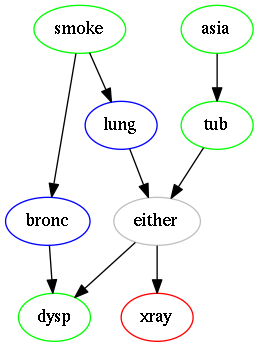
\includegraphics[scale=0.5]{images/reach_lung_bronc_giv_either.png}
\caption{Alcançáveis em relação a \texttt{lung} e \texttt{bronc} dado \texttt{either}}
\label{fig:alcanc}
\end{figure}

Alguns exemplos de uso do método \verb|is_d_separated| são dados abaixo.

\begin{verbatim}
In [5]: import bayesnet as bn
In [6]: net4_1 = bn.BayesNet.init_from_bif_file('../examples/dseparation/ex4.1/ex4.1.bif')
In [8]: net4_1.is_d_separated(['A'], ['E'], ['B', 'H'])
Out[8]: False
In [9]: net4_1.is_d_separated(['G'], ['E'], ['D'])
Out[9]: False
In [10]: net4_1.is_d_separated(['A', 'B'], ['G', 'H'], ['F'])
Out[10]: False
\end{verbatim}

Compare os resultados obtidos com os grafos pintados de acordo com a acessibilidade dos nós nas Figuras~\ref{fig:alcancA_BH},~\ref{fig:alcancG_D}, e~\ref{fig:alcancAB_F}.

\begin{figure}[hbtp]
\centering
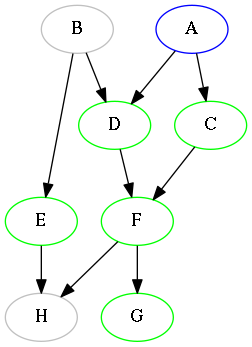
\includegraphics[scale=0.5]{images/net4_1_A_giv_BH.png}
\caption{A partir de \texttt{A} dados \texttt{B, H}}
\label{fig:alcancA_BH}
\end{figure}
\begin{figure}[hbtp]
\centering
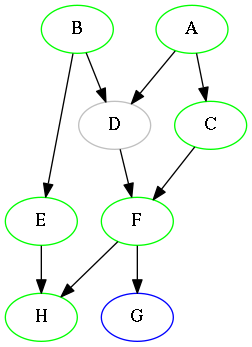
\includegraphics[scale=0.5]{images/net4_1_G_giv_D.png}
\caption{A partir de \texttt{G} dado \texttt{D}}
\label{fig:alcancG_D}
\end{figure}
\begin{figure}[hbtp]
\centering
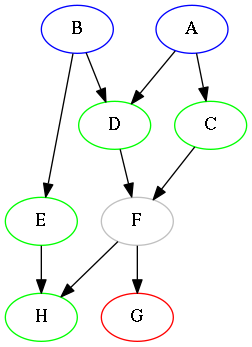
\includegraphics[scale=0.5]{images/net4_1_AB_giv_F.png}
\caption{A partir de \texttt{A, B} dado \texttt{F}}
\label{fig:alcancAB_F}
\end{figure}

\end{document}
